\chapter[Modèle de Riesz]{Étude théorique du modèle de Riesz} % signal monogénique ?
\label{chap:chapitre3}

Dans le but de synthétiser du contenu avec de la structure irrégulière, nous cherchons à avoir une approche locale. Pour cela nous utilisons le modèle du signal monogénique \cite{felsberg_monogenic_2001}, qui permet d'extraire l'énergie locale, en s'appuyant sur la transformée de Riesz. Ce SY procédé est ensuite mis en application dans un cadre multi-résolutionnel, les pyramides de Riesz \cite{wadhwa_riesz_2014}, pour calculer la congruence de phases.

\section{Signal monogène}

Le signal monogène est un outil du domaine du traitement du signal, généralement utilisé pour des tâches d'analyse d'image ou de vision par ordinateur, comme la détection de caractéristiques. La revue de la méthode par Bridge \cite{bridge_introduction_2018} est une bonne introduction aux principes théoriques du signal monogène ; nous reprennons dans cette partie sa notation et son discours exposé dans son document afin de prodiguer une compréhension du modèle.

\subsection{Une dimension, signal analytique}

\subsubsection{Construction du singal analytique}

Pour comprendre l'utilité du signal monogène, commençons par expliquer le fonctionnement du signal analytique, dont le signal monogène est l'extension aux signaux de dimension arbitraire. Le signal analytique est une méthode de représentation d'un signal 1D à valeurs réelles, qui facilite la manipulation et l'extraction de certaines informations du signal original. Le constat qui donne lieu à cette représentation est que pour un signal à valeurs réelles, les fréquences négatives sont superflues pour sa représentation de Fourier. En effet, on rappelle que la transformée de Fourier $F(\omega)$ d'un signal à valeurs réelles $f(t)$ présente une symétrie hermitienne :

\begin{equation}
    F(-\omega) = \overline{F(\omega)}
\end{equation}

avec $\overline{\cdot}$ l'opérateur de conjugaison complexe. L'idée est donc de se débarrasser des fréquences négatives, sans perte d'information, et de construire un nouveau signal en n'utilisant que les fréquences positives de $f(t)$. On exprime d'abord le signal $F_{\alpha}$ dans le domaine de Fourier :

\begin{equation}
    F_{\alpha}(\omega) = \left\{
    \begin{array}{ll}
        2F(\omega), & \omega > 0 \\
        0, & \omega < 0 \\
        F(0), & \omega = 0,
    \end{array}
    \right.
\end{equation}

où l'amplitude des composantes de fréquences positives est doublée, par soucis de conservation d'énergie. Avec cette formulation, toute l'information de notre signal original est conservée, mais cette nouvelle forme permet de faire des manipulations précédemment impossibles qui nous permettent de mieux comprendre notre signal.

\begin{figure}[h]
    %\noindent
    \hspace{-12pt}
    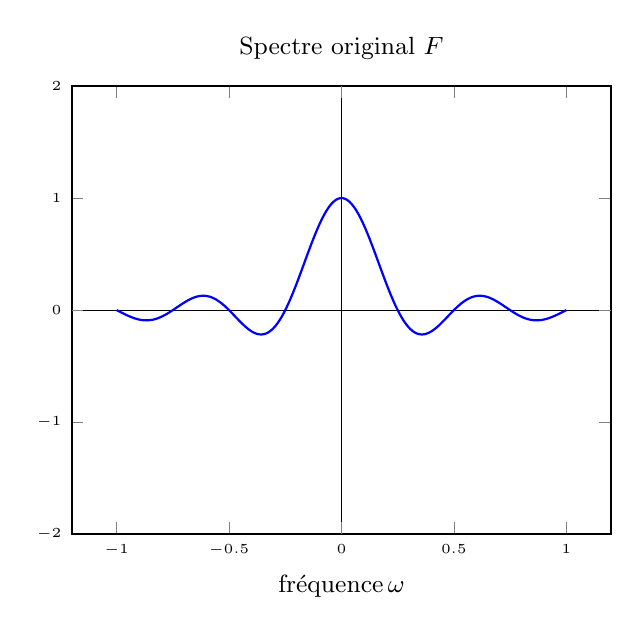
\begin{tikzpicture}
    \begin{axis}[
        title={Spectre original $F$},
        title style={font=\small},
        axis lines=box,
        style=thick,
        xlabel=\(\textnormal{fréquence}\, \omega\),
        xtick={-1, -0.5, 0.5, 1},
        ytick={-2, -1, 1, 2},
        extra x ticks=0,
        extra y ticks=0,
        extra x tick style={grid=major, grid style={black}},
        extra y tick style={grid=major, grid style={black}},
        tick label style={font=\tiny},
        label style={font=\small},
        ymin=-2, 
        ymax=2,
        ]
    \addplot[
        color=blue,
        domain=-1:1,
        samples=200
        ]
    {sin(360*x*2)/ (2*pi*x*2)};
    \end{axis}
    \end{tikzpicture}
    %\hskip 6pt
    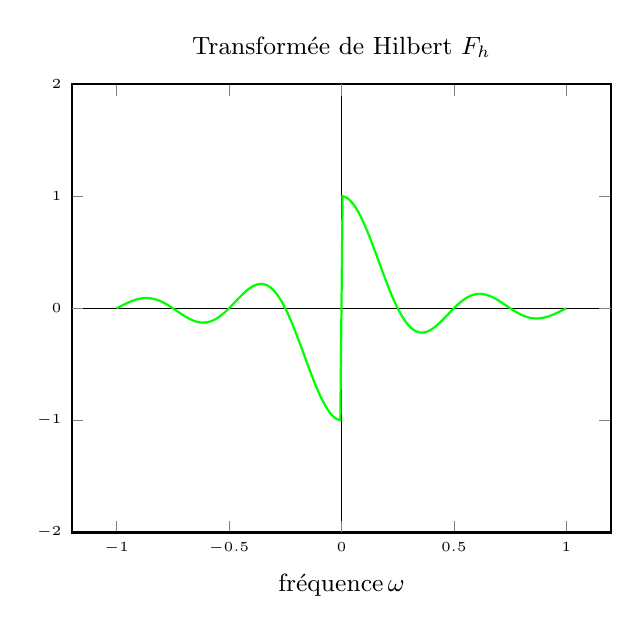
\begin{tikzpicture}
    \begin{axis}[
        title={Transformée de Hilbert $F_h$},
        title style={font=\small},
        axis lines=box,
        style=thick,
        xlabel=\(\textnormal{fréquence}\, \omega\),
        xtick={-1, -0.5, 0.5, 1},
        ytick={-2, -1, 1, 2},
        extra x ticks=0,
        extra y ticks=0,
        extra x tick style={grid=major, grid style={black}},
        extra y tick style={grid=major, grid style={black}},
        tick label style={font=\tiny},
        label style={font=\small},
        ymin=-2, 
        ymax=2,
        ]
    \addplot[
        color=green,
        domain=-1:1,
        samples=200
        ]
    {sign(x)*sin(360*x*2)/ (2*pi*x*2)};
    \end{axis}
    \end{tikzpicture}
    %\hskip 6pt
    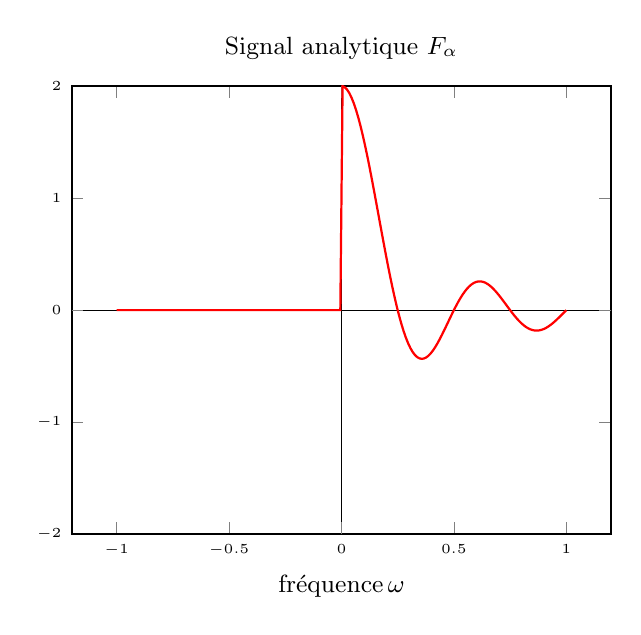
\begin{tikzpicture}
    \begin{axis}[
        title={Signal analytique $F_{\alpha}$},
        title style={font=\small},
        axis lines=box,
        style=thick,
        xlabel=\(\textnormal{fréquence}\, \omega\),
        xtick={-1, -0.5, 0.5, 1},
        ytick={-2, -1, 1, 2},
        extra x ticks=0,
        extra y ticks=0,
        extra x tick style={grid=major, grid style={black}},
        extra y tick style={grid=major, grid style={black}},
        tick label style={font=\tiny},
        label style={font=\small},
        ymin=-2, 
        ymax=2,
        ]
    \addplot[
        color=red,
        domain=-1:1,
        samples=200
        ]
    {(1+sign(x))*sin(360*x*2)/ (2*pi*x*2)};
    \end{axis}
    \end{tikzpicture}

    \captionof{figure}{Création du signal analytique dans le domaine fréquentiel (seule la partie réelle est montrée). Le signal original réel (gauche), qui présente une symétrie hermitienne, est ajouté à sa transformée de Hilbert (milieu), lui impair, pour former le signal analytique (droite), dépourvu de fréquence négative.}
    \label{fig:complex-analytic-representation}
\end{figure}

En effet, on peut voir le fait de supprimer les composantes de fréquences négatives comme le l'ajout d'un signal impair soigneusement choisi au signal de base.

\begin{equation} \label{eq:2.1}
    F_{\alpha}(\omega) = F(\omega) + F_h(\omega),
\end{equation}

où $F_h(\omega)$ est la « version impaire » du signal $F(\omega)$ :

\begin{equation}
    F_h(\omega) = \left\{
    \begin{array}{ll}
        F(\omega), & \omega > 0 \\
        -F(\omega), & \omega < 0 \\
        0, & \omega = 0,
    \end{array}
    \right.
\end{equation}

que l'on peut reformuler à l'aide de la fonction signe $\sgn$ :

\begin{equation}
    F_h(\omega) = F(\omega)\cdot \sgn(\omega).
\end{equation}

On rappelle l'expression de la fonction signe :

\begin{equation}
    \sgn(x) = \left\{
    \begin{array}{ll}
        1, & x > 0 \\
        -1, & x < 0 \\
        0, & x = 0.
    \end{array}
    \right.
\end{equation}

On obtient alors la ré-écriture de l'équation \ref{eq:2.1} :

\begin{equation}
    F_{\alpha}(\omega) = (1+\sgn(\omega))F(\omega)
\end{equation}

\begin{figure}[h]
    %\noindent
    %\hspace{-10pt}
    \centering
    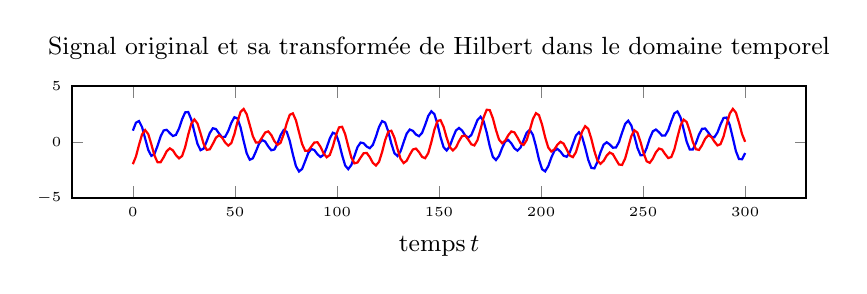
\begin{tikzpicture}
    \begin{axis}[
        title={Signal original et sa transformée de Hilbert dans le domaine temporel},
        title style={font=\small},
        axis lines=box,
        width=0.9\textwidth,
        height=3cm,
        style=thick,
        xlabel=\(\textnormal{temps}\, t\),
        xtick={0, 50, 100, 150, 200, 250, 300},
        ytick={-5, 0, 5},
        tick label style={font=\tiny},
        label style={font=\small},
        ymin=-5, 
        ymax=5,
        ]
    \addplot[
        color=blue,
        domain=0:300,
        samples=200
        ]
    {sin(3*x)+cos(15*x)+sin(30*x)};
    \addplot[
        color=red,
        domain=0:300,
        samples=200
        ]
    {-cos(3*x)+sin(15*x)-cos(30*x)};
    \end{axis}
    \end{tikzpicture}

    \captionof{figure}{Exemple de représentation analytique. Le signal original réel (en bleu), et sa transformée de Hilbert imaginaire pure (en rouge).}
    \label{fig:analytic-representation}
\end{figure}


Le signal $F_{\alpha}$ créé est donc dans le domaine fréquentiel de $F$, signal original pair, de représentation purement réelle dans le domaine temporel, et de $F_h$, signal impair, de représentation purement imaginaire dans le domaine temporel, que l'on nomme $f_h$. Dans le domaine temporel, $f_{\alpha}$ est donc un signal complexe, sans composantes de fréquences négatives, c'est un signal analytique, que l'on appelle la \textit{représentation analytique} de $f$ :

\begin{equation}
    f_{\alpha}(t) = \underbrace{f(t)}_\text{réel pur} + \underbrace{f_h(t)}_\text{imaginaire pur}.
\end{equation}

Le signal ajouté pour annuler les fréquences $F_h$ est par ailleurs un objet connu : c'est la \textit{transformée de Hilbert} de $F$. Sa représentation, bien que très simple dans le domaine fréquentiel, est difficile à obtenir et manipuler dans le domaine temporel :

\begin{equation}
    f_h(t) = i \cdot \textnormal{p.v.} \int_{-\infty}^{\infty} \frac{f(t)}{\pi(t-\tau)} \,d\tau,
\end{equation}

où p.v. est la valeur principale de Cauchy, nécessaire pour cette intégrale, qui représente la convolution avec la distribution $\frac 1{\pi t}$ et qui est impropre à cause de la singularité en $t=\tau$. Cependant, dû à la complexité de cet objet, nous utiliserons majoritairement l'expression fréquentielle de la transformée de Hilbert :

\begin{align*}
    &\hil(F) = F_h = \sgn\cdot F \\
    &\mathcal{H}(F) = F_h = \sgn\cdot F
\end{align*}


\subsubsection{Amplitude et phase locales}

Pour comprendre l'intérêt du signal analytique, on étudie d'abord l'exemple d'une fonction sinusoïdale, d'amplitude $A$ et de fréquence $\omega_0$ fixées :

\begin{equation}
    f(t) = A\sin(\omega_0t).
\end{equation}

En utilisant les relations montrées précédemment, on trouve la transformée de Hilbert de $f$ et on calcule sa représentation analytique :

\begin{align}
    f_h(t) &= iA\cos(\omega_0t) \\
    f_{\alpha}(t) &= f(t) + f_h(t) \\
    &= A\sin(\omega_0t)+iA\cos(\omega_0t) \\
    &= Ae^{i\omega_0t}.
\end{align}

Pour une sinusoïde, la transformée de Hilbert est un simple \textit{déphasage} de $-\frac{\pi}2$ du signal original. Or la théorie de Fourier nous indique que n'importe quel signal générique peut être décomposé comme une somme de sinusoïdes. Ainsi la transformée de Hilbert agit de la même manière sur tous les signaux : c'est un déphasage de $-\frac{\pi}2$ de chaque composante fréquentielle qui compose le signal. Le signal $f$ et sa transformée de Hilbert $f_h$ sont dit en \textit{quadrature de phase}, et le signal analytique s'exprime comme une exponentielle complexe.

\bigskip

En fait, puisque tout signal est maintenant représenté comme la somme d'un réel et d'un imaginaire pur, on peut toujours l'exprimer en coordonnées polaires comme une exponentielle complexe, d'amplitude et phase variant au cours du temps :

\begin{equation}
    f_{\alpha} (t) = A(t)e^{i\phi(t)}.
\end{equation}

avec 

\begin{align}
    A(t) &= \sqrt{f(t)^2 + h_h(t)^2} \\
    \phi(t) &= \arctan\left(\frac{f_h(t)}{f(t)}\right).
\end{align}

Cette représentation introduit le concept d'\textit{amplitude locale} et de \textit{phase locale} (ici \textit{temporellement} locales), qui sont deux outils d'analyse particulièrement intéressants pour l'étude approfondie du signal original. L'amplitude locale agit comme une mesure de l'\textit{enveloppe} du signal, et la phase locale comme une mesure de la \textit{forme} du signal. Par exemple, une phase de $0$ indique un extremum, et une phase de $\pm\pi$ indique un passage par zéro. La figure \ref{fig:local-pha-amp} montre un signal avec son amplitude locale et sa phase locale. À partir uniquement de notre signal initial, on a ainsi créé un outil nous permettant d'obtenir de l'information bien plus intéressante sur l'apparence et les propriétés du signal.

\begin{figure}[h]

    \centering
    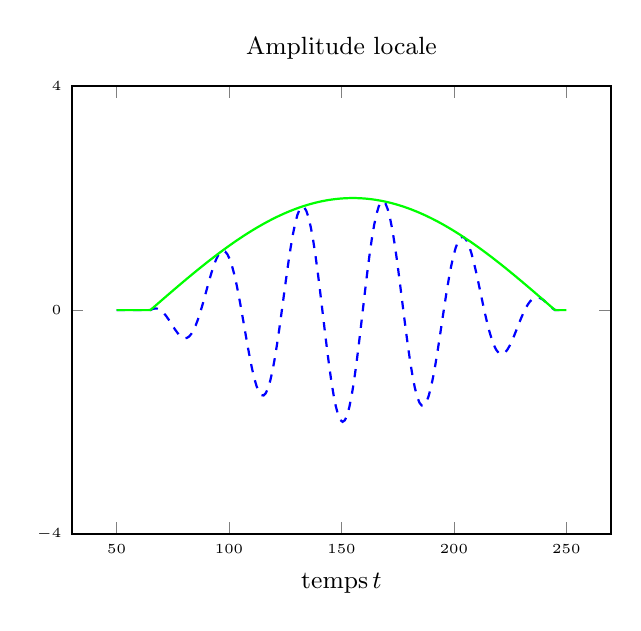
\begin{tikzpicture}
    \begin{axis}[
        title={Amplitude locale},
        title style={font=\small},
        axis lines=box,
        %width=0.9\textwidth,
        %height=3cm,
        style=thick,
        xlabel=\(\textnormal{temps}\, t\),
        xtick={50, 100, 150, 200, 250},
        ytick={-4, 0, 4},
        tick label style={font=\tiny},
        label style={font=\small},
        ymin=-4, 
        ymax=4,
        ]
    \addplot[
        color=blue,
        domain=50:250,
        samples=200,
        style=dashed,
        ]
    {(sign(x-65)-sign(x-245))*sin(10*x+25)*cos(x+25)};
    \addplot[
        color=green,
        domain=50:250,
        samples=200
        ]
    {(sign(x-65)-sign(x-245))*sqrt((0.5*(sin(11*x-40) + sin(9*x-90)))^2 + (sin(10*x+25)*cos(x+25))^2)};
    \end{axis}
    \end{tikzpicture}
    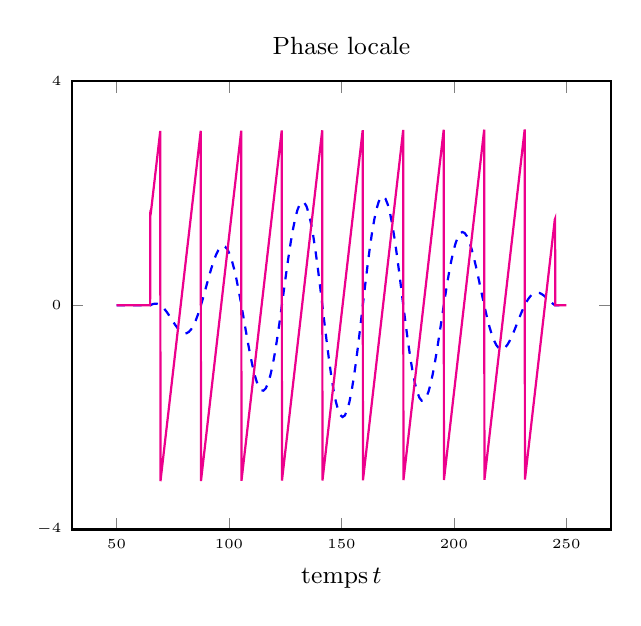
\begin{tikzpicture}
    \begin{axis}[
        title={Phase locale},
        title style={font=\small},
        axis lines=box,
        %width=0.9\textwidth,
        %height=3cm,
        style=thick,
        xlabel=\(\textnormal{temps}\, t\),
        xtick={50, 100, 150, 200, 250},
        ytick={-4, 0, 4},
        tick label style={font=\tiny},
        label style={font=\small},
        ymin=-4, 
        ymax=4,
        ]
    \addplot[
        color=blue,
        domain=50:250,
        samples=200,
        style=dashed,
        ]
    {(sign(x-65)-sign(x-245))*sin(10*x+25)*cos(x+25)};
    \addplot[
        color=magenta,
        domain=50:250,
        samples=2000
        ]
    {(sign(x-65)-sign(x-245))*rad(atan((0.5*(sin(11*x-40) + sin(9*x-90))) / (sin(10*x+25)*cos(x+25))))};
    \end{axis}
    \end{tikzpicture}

    \caption{Extraction d'informations locales pour un cosinus modulé par un sinus. L'amplitude locale (gauche) donne l'enveloppe de la sinusoïde, et la phase locale (droite) nous donne de l'information quant à la position dans le cycle d'oscillation.}
    \label{fig:local-pha-amp}

\end{figure}

\subsubsection{Notion d'échelle}

L'exemple donné avec la figure \ref{fig:local-pha-amp} fonctionne bien car le signal est simple, l'interprétation de l'amplitude et la phase locale est claire et visuelle. Pour un signal plus complexe, plus représentatif des signaux que l'on doit souvent étudier, ce n'est pas si facile. La figure \ref{fig:complex-local-pha-amp} affiche les informations locales du signal de la figure \ref{fig:analytic-representation}, une somme de trois sinusoïdes de fréquences différentes ; il est moins évident de comprendre ce que les informations locales représentent dans ce cas.

\begin{figure}[h]
    \centering
    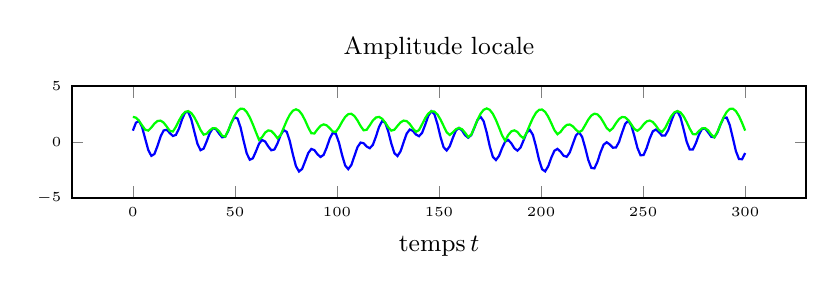
\begin{tikzpicture}
    \begin{axis}[
        title={Amplitude locale},
        title style={font=\small},
        axis lines=box,
        width=0.9\textwidth,
        height=3cm,
        style=thick,
        xlabel=\(\textnormal{temps}\, t\),
        xtick={0, 50, 100, 150, 200, 250, 300},
        ytick={-5, 0, 5},
        tick label style={font=\tiny},
        label style={font=\small},
        ymin=-5, 
        ymax=5,
        ]
    \addplot[
        color=blue,
        domain=0:300,
        samples=200
        ]
    {sin(3*x)+cos(15*x)+sin(30*x)};
    \addplot[
        color=green,
        domain=0:300,
        samples=200
        ]
    {sqrt((sin(3*x)+cos(15*x)+sin(30*x))^2 + (-cos(3*x)+sin(15*x)-cos(30*x))^2)};
    \end{axis}
    \end{tikzpicture}
    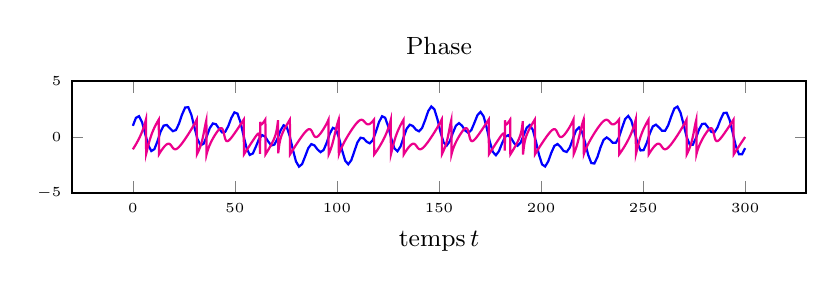
\begin{tikzpicture}
    \begin{axis}[
        title={Phase},
        title style={font=\small},
        axis lines=box,
        width=0.9\textwidth,
        height=3cm,
        style=thick,
        xlabel=\(\textnormal{temps}\, t\),
        xtick={0, 50, 100, 150, 200, 250, 300},
        ytick={-5, 0, 5},
        tick label style={font=\tiny},
        label style={font=\small},
        ymin=-5, 
        ymax=5,
        ]
    \addplot[
        color=blue,
        domain=0:300,
        samples=200
        ]
    {sin(3*x)+cos(15*x)+sin(30*x)};
    \addplot[
        color=magenta,
        domain=0:300,
        samples=3000
        ]
    {rad(atan((-cos(3*x)+sin(15*x)-cos(30*x)) / (sin(3*x)+cos(15*x)+sin(30*x))))};
    \end{axis}
    \end{tikzpicture}    

    \caption{Caption}
    \label{fig:complex-local-pha-amp}
\end{figure}

Le problème à l'analyse de ce signal est le fait qu'il existe plusieurs niveaux de structure, qui interfèrent et rendent l'interprétation des informations locales impossible à l'échelle macroscopique.
Pour extraire de l'information utile, il faut sélectionner et faire l'analyse d'un seul niveau de structure, donc d'échelle.
Pour cela, on filtre les composantes des niveaux qui ne nous intéressent pas.
Pour se faire, il est possible d'utiliser des filtres passe-bande, comme le fait Bridge avec les filtres log-Gabor, un choix commun pour ce genre de pratique.
Un filtre log-Gabor est un filtre défini dans le domaine fréquentiel, qui permet de sélectionner une bande de fréquence centrée autour d'une fréquence centrale $\omega_0$.
Il a une réponse en fréquence de forme gaussienne quand observé en échelle logarithmique :

\begin{equation}
    G(\omega) = \exp\left(-\frac{\log^2(\frac{|\omega|}{\omega_0})}{2\log(\sigma_0)^2}\right).
\end{equation}

Ces filtres sont caractérisés par deux paramètres : la fréquence centrale $\omega_0$, qui contrôle quelle échelle de structure est sélectionnée, et la largeur de bande $\sigma_0$, un paramètre de forme qui contrôle la largeur de la bande de fréquence sélectionnée. Des exemples de filtre log-Gabor sont montrés à la figure \ref{fig:log-gabor-filters}.

En appliquant un filtre log-Gabor à notre signal avant de lui appliquer la transformée de Hilbert et de déterminer sa représentation analytique, on obtient une représentation locale du signal, centrée autour d'une fréquence $\omega_0$ et d'une échelle $\sigma_0$ que l'on peut faire varier arbitrairement.

\begin{equation}
    F_{\alpha}(\omega) = (1+\sgn(\omega))G(\omega)F(\omega)
\end{equation}

\begin{figure}
    \centering
    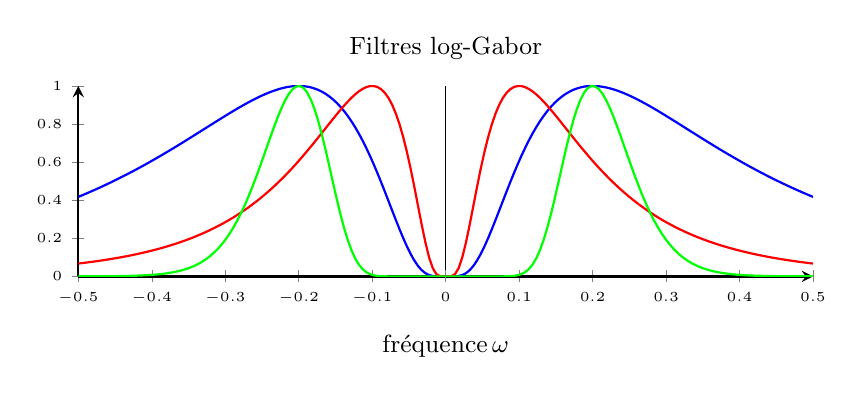
\begin{tikzpicture}
    \begin{axis}[
        title={Filtres log-Gabor},
        title style={font=\small},
        axis lines=left,
        width=0.9\textwidth,
        height=4cm,
        style=thick,
        xlabel=\(\textnormal{fréquence}\, \omega\),
        xtick={-0.5, -0.4, -0.3, -0.2, -0.1, 0.1, 0.2, 0.3, 0.4, 0.5},
        ytick={0, 0.2, 0.4, 0.6, 0.8, 1},
        tick label style={font=\tiny},
        label style={font=\small},
        extra x ticks=0,
        extra x tick style={grid=major, grid style={black}},
        ymin=0,
        ymax=1,
        ]
    \addplot[
        color=blue,
        domain=-0.5:0.5,
        samples=200
        ]
    {exp(-ln(abs(x)/.2)^2 / (2*ln(.5)^2))};
    \addplot[
        color=red,
        domain=-0.5:0.5,
        samples=200
        ]
    {exp(-ln(abs(x)/.1)^2 / (2*ln(.5)^2))};
    \addplot[
        color=green,
        domain=-0.5:0.5,
        samples=200
        ]
    {exp(-ln(abs(x)/.2)^2 / (2*ln(.8)^2))};
    \end{axis}
    \end{tikzpicture}

    \caption{Représentation dans le domaine fréquentiel de filtres log-Gabor de différents paramètres. En rouge, $\omega_0=0.1, \sigma_0 = 0.5$. En bleu, $\omega_0=0.2, \sigma_0 = 0.5$. En vert, $\omega_0=0.2, \sigma_0 = 0.8$.}
    \label{fig:log-gabor-filters}
\end{figure}

En étudiant la réponse du signal sur une large gamme de fréquences et d'échelles, on obtient une représentation locale du signal à différentes échelles, et ainsi extraire de l'information sur les différentes structures du signal. On peut rassembler toutes ces informations dans un graphique appelé scalogramme, qui représente le comportement de la phase locale en fonction du temps et de l'échelle, comme montré à la figure~\ref{fig:scalogram}. On y voit facilement les différents niveaux de structure du signal, et l'interprétation des informations locales devient plus utile car on peut choisir à quel niveau on regarde.

Si l'on compare le modèle du signal analytique à celui de la transformée de Fourier, on remarque que les informations que l'on obtient avec les deux diffèrent et se complètent. La transformée de Fourier nous donne de l'information globale sur tout le signal, mais localisée en termes de fréquence. La représentation analytique, elle, nous donne une information spatialement locale sur le signal, mais sur une bande de fréquences, sélectionnées par un filtre passe-bande. Le modèle d'information locale est donc un compromis entre la localisation spatiale et fréquentielle, et permet d'obtenir une information différente sur le signal.


\begin{figure}
    \centering
    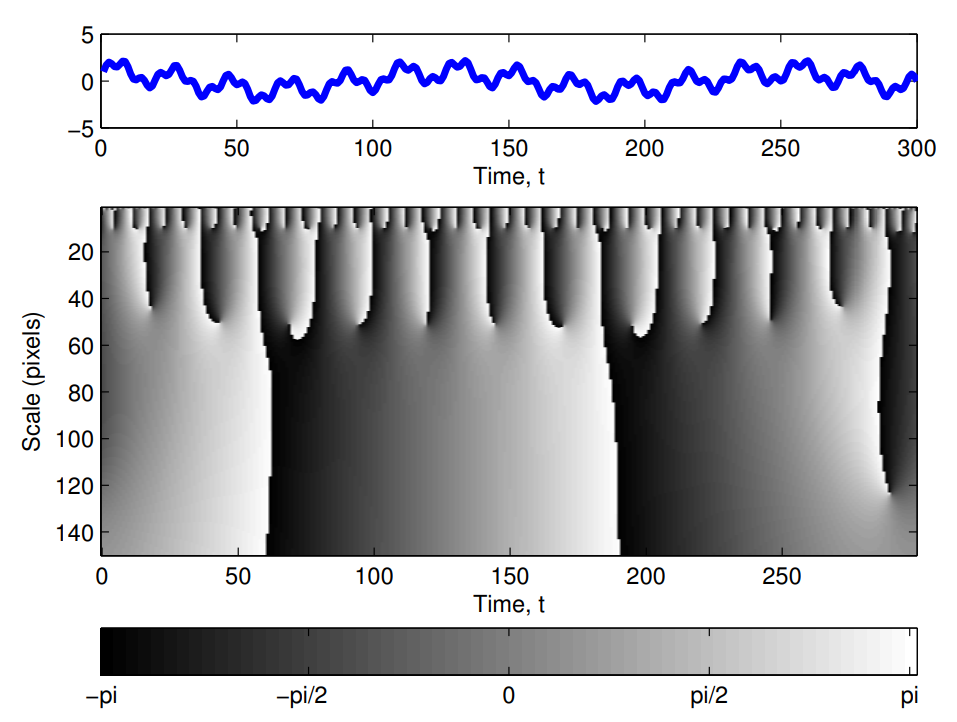
\includegraphics[width=\textwidth]{contenu/resources/images/scalogram}
    \caption{Scalogramme de la phase locale pour un signal complexe. La phase locale est représentée en échelle de gris, et varie en fonction du temps (en abscisse) et de l'échelle en nombre de pixels (en ordonnée). Diagramme par Bridge~\cite{bridge_introduction_2018}.}
    \label{fig:scalogram}
\end{figure}


\subsection{Deux dimensions, signal monogène}

Le modèle du signal analytique est utile à l'extraction d'informations locales pour des signaux 1D, et il serait intéressant d'avoir accès à ces informations pour des images, donc des signaux 2D. En effet l'importance de la phase dans l'analyse d'image a déjà été soulignée depuis longtemps~\cite{oppenheim_importance_1981}. Cependant, l'application n'est pas directe dans le cas de deux (ou plus) dimensions, car il y a une notion de direction à considérer. C'est ce que le modèle du signal monogène, proposé par Felsberg et Sommer~\cite{felsberg_monogenic_2001}, permet de faire, que nous allons développer dans cette partie.

\subsubsection{Construction du signal monogène}



\section{Transformée de Riesz}

\section{Pyramide de Riesz}
